\begin{figure}[ht]
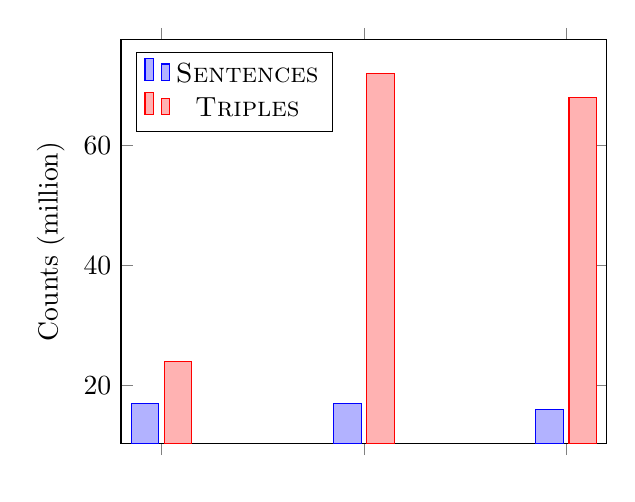
\begin{tikzpicture}
\begin{axis}[
    scale=0.9,
    ybar, 
    xtick=data,
    legend pos=north west,
    ylabel=Counts (million),
    xticklabels={
      \reverb, \openie, \openiecoref
    },
]
\addplot 
    coordinates {(1,17) (2,17) (3,16)};
            \addlegendentry{\textsc{Sentences}}

\addplot 
    coordinates {(1,24) (2,72) (3,68)};
            \addlegendentry{\textsc{Triples}}

\end{axis}
\end{tikzpicture}
  \caption{
    \label{fig:extrapolated}
    Results from \reftab{raw_counts}, except we linearly
    extrapolate the \openiecoref{} counts using a rate of
    $532/513=1.037$ to account for the difference in 
    number of articles successfully processed.
  }
\end{figure}
